
\section{Background}
\label{sec:bg}

DAG task scheduling introduces several fundamental concepts.

%\subsection{Periodic task and schedule}
%~
%
%Firstly, a periodic task $\tau_i(C_i, D_i, T_i)$ is characterized 
%by its worst-case execution time (wcet) $C_i$, its deadline $D_i$, and 
%its period $T_i$. This definition can be expanded by including an 
%initial offset, which corresponds to the time of the task's first 
%execution, and an activation offset, which is the time delay between 
%the task being ready to execute (i.e., its execution period has begun) 
%and the task actually starting to run. Secondly, a schedule $S$ is a 
%function that assigns a boolean value for each task $\tau$ and each 
%time tick $t$, indicating whether the task $\tau$ is running at 
%time $t$. Therefore, a scheduling algorithm is the method that, 
%given a set of tasks, produces a schedule $S$ for the task set.
%
%This task model and schedule definition are widely adopted in the literature (see section \ref{sec:literature}) 
%and are the building blocks of all scheduling algorithms.
%The periodic task model, in particular, is used to define more complex
%tasks such as DAG tasks (see below) that will be used as input in the 
%machine learning model (see section \ref{sec:methodology}).

\subsection{DAG task model}
~

A Directed Acyclic Graph (DAG) task
$\tau = (G, D, T)$ is comprised of 
a directed acyclic graph $G = (V, E)$, a relative deadline $D > 0$ and a period $T > 0$.
The graph $G$ has a set of vertices $V$ and a set of edges $E \subseteq V \times V$
that models the precedence constraints of the vertices,
i.e., for all $(v_i, v_j) \in V^2$, with $i \neq j$, $(v_i, v_j) \in E$ if and only if
$v_j$ must wait the end of $v_i$'s execution to start executing(i.e., $v_i$ is a precedence constraint for $v_j$).
The nodes of the graph $G$ are characterized by their own worst-case execution time $C_{v_i}$ 
and $vol(G) = \sum_{v_i \in V} C_{v_i}$ is the worst-case execution time of the DAG task $\tau$,
also called the total workload of the DAG task.
A \textit{source} node is the node which only has successors 
and no predecessors, and a \textit{sink} node is 
the node that only has predecessors and no sucessors.
It is assumed that all DAGs have a unique source node and a unique sink node.
This can always be assumed as you can always add a dummy sink or source node,
setting their wcet to 0,
at the end or beginning of a DAG that has multiple sink or source nodes,
linking those non-unique sink and source nodes to
the dummy nodes added so that the dummy nodes become the unique source node and sink node
of the DAG.
In this paper, the words nodes, vertices and subtasks will be used
to address the same thing, that is the vertices of the graph of a DAG task.\\

An example of a DAG task is shown in Figure \ref{fig:dag_example},
where the DAG task has a wcet of 24 time units.

\begin{figure}[htbp]
    \centering
    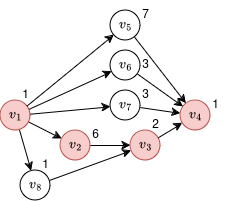
\includegraphics[width=0.5\linewidth]{images/example_DAG.png}
    \caption{DAG task $\tau$. The worst-case execution time (wcet) of each subtask is written as an exponent
    and the nodes highlighted in red are the nodes in the critical path, the path of maximum length in terms of wcets.}
    \label{fig:dag_example}
    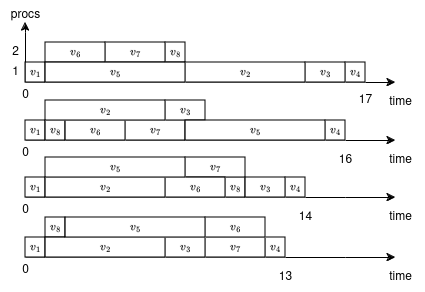
\includegraphics[width=\linewidth]{images/example_DAG_schedules.png}
    \caption{Execution schedules for the DAG task above. Heavily inspired from \citet{zhao2020DAGsched}.}
    \label{fig:dag_schedule_example}
\end{figure}


The DAG task model will be the task model used in order to conduct 
the systematic literature review (see Section \ref{sec:literature})
and it will also be the task model used for designing 
the supervised machine learning model (see Section \ref{sec:methodology}).

\subsection{Makespan}

The makespan or end-to-end response time of a 
DAG task is the amount of time it takes for all the subtasks
in the DAG task to finish executing when given a schedule.
For instance, for the task $\tau$ shown in Figure \ref{fig:dag_example},
the makespan of $\tau$ for the first schedule (from top to bottom) shown in Figure \ref{fig:dag_schedule_example}
is 17.
Notice that Figure \ref{fig:dag_schedule_example} shows multiple
ways of scheduling the DAG task, the bottom one yielding a makespan of 13.

This is a key measurement when scheduling the nodes of a single DAG task,
also called intra-task scheduling (see Section \ref{sec:literature}),
and it will be the main efficacy criteria when comparing 
the machine learning model with state-of-the-Art heuristics and ILP
(see Section \ref{sec:methodology}).

\subsection{Intra-task and inter-task scheduling}
~

When considering the DAG task model,
two concepts arise: intra-task scheduling and inter-task scheduling.
Intra-task scheduling of DAG tasks is when only the execution
order of the nodes in a single DAG task is considered.
The goal of such a problem being to minimize the makespan
of a single DAG task.

Inter-task scheduling, on the other hand, is when multiple DAG tasks
are considered and the goal then becomes to maximize the acceptance ratio (see below)
of the scheduling algorithm.

\subsection{NP-hardness intuition and problem motivation}
~

The problem of intra-task scheduling of DAG tasks,
that is, scheduling the nodes of a single DAG task so that 
the makespan is minimized,
is a NP-hard problem\cite{ULLMAN1975NPhard}\cite{du1989schedNPhard}
but can also be intuitively seen as a NP-hard problem when looking at 
the schedules shown in Figure \ref{fig:dag_schedule_example}.
Indeed, 
when looking at a single DAG task,
a simple yet efficient way of scheduling the nodes 
is looking at a critical-path-first execution order(CPFE).
The critical path, highlighted in red in Figure \ref{fig:dag_example},
is the longest path of the graph in terms of wcets.
The CPFE principle is applied in the third schedule (from top to bottom)
in Figure \ref{fig:dag_schedule_example} and achieves a makespan of 14.
But this is not the minimum makespan as the fourth schedule yields a makespan
of 13.

This is due to the fact that, although executing the critical path first
is the best strategy\cite{zhao2020DAGsched}, 
one needs to take into account the dependency constraints
and thus the global structure of the graph.
The fourth schedule in Figure \ref{fig:dag_schedule_example}
achieves a makespan of 13 by prioritizing the execution of node $v_8$
before node $v_5$ which is crucial to enable $v_3$ to execute sooner
than in the third schedule.
Typically in graph theory, when the global structure needs to be known 
in advance
in order to find the best solution, it often means that the problem is NP-hard
(e.g., the problem of coloring a graph\cite{book1975richardNPhardColorGraph}
or coloring a path of a graph\cite{ERLEBACH2001ColorPathNPhard}).
Therefore, researchers have resorted to heuristics to compute an execution order
that minimizes the bound of the DAG, reducing its wcet 
by providing a better worst-case makespan bound than $vol(G)$ (see Section \ref{sec:literature}).


\subsection{Utilization factor}

The utilization factor represents the percentage of processing 
time that a taskset $(\tau_1, \cdots, \tau_n)$ will utilize. 
Formally, it is defined as
\begin{align}
U = \sum_{k=1}^{n} \frac{vol(G_k)}{T_k}
\end{align}
where $U$ is the utilization factor. This concept is significant 
because, when evaluating a scheduling algorithm $S$, we desire 
$S$ to effectively schedule tasksets that maximize the utilization 
factor $U$. Consequently, the higher the utilization factor bound 
for $S$, the more efficient the scheduling algorithm. Additionally, 
this concept is valuable in real-time systems where processing 
resources are often limited and expensive, making it crucial to 
maximize their usage.

This concept is also used either as a measurement
when comparing two scheduling algorithms 
and considering their utilization bound,
or used as a parameter to generate tasksets or DAG tasks with 
a fixed utilization (see Section \ref{sec:literature}).

\subsection{Capacity augmentation bound}

Another measurement used when scheduling DAG tasks  
is the capacity bound, or capacity augmentation bound,
which compares resource use to a theoretically optimal scheduling algorithm.
It can also be used as a simple schedulability test.
It is often refer to as a $\beta$ coefficient and the lower $\beta$ is, the better the scheduling algorithm.\\
This metric is used in the literature when scheduling DAG tasks (Section \ref{sec:literature}).

%\cite{tiryaki2006sunit} is really good with MAS but really bad with something else.
%\subsection{Optimality}
%
%A scheduling algorithm $S$ is said to be optimal 
%when the following condition is true:
%for every taskset $\Omega$, if there exists 
%a scheduling algorithm $S'$ so that $\Omega$ is feasible by $S'$,
%then $\Omega$ is also feasible by $S$.
%Where {\it{feasible}}, 
%means that, using the schedule generated by $S$,
%all the tasks in the taskset will finish executing before their deadlines.
%
%This concept is used in the literature, mainly for independent tasks scheduling
%(see Section \ref{sec:literature}).

\subsection{Acceptance ratio}

When dealing with several independent DAG tasks
or tasksets, 
the acceptance ratio is often used to measure the 
performance of a scheduling algorithm (see Section \ref{sec:literature}).
It consists of looking at a number of generated tasksets (or DAG tasks)
and calculating the amount of schedulable (i.e., 
the schedule produced doesn't lead to a deadline miss) tasksets compared to 
the total amount of taskets.
The resulting percentage is the acceptance ratio 
and the closer it gets to 100\% for a given scheduling algorithm, the better the scheduling algorithm.

This concept is thus used as a metric, to assert the efficiency
of scheduling algorithms when considering inter-task scheduling (see Section \ref{sec:literature}).
\\


While the acceptance ratio, also called system schedulability, is used 
to measure the performance of scheduling algorithms for inter-DAG task scheduling
(i.e., scheduling multiple DAG tasks),
the makespan and the capacity bound are only used for single DAG tasks.

%\subsection{RM and EDF scheduling}
%~
%
%When designing a scheduling algorithm, the key decision involves 
%determining which task should execute first when two or more 
%independent tasks are ready to execute. This requires assigning each 
%task a priority. \cite{liu1973scheduling} introduced two 
%heuristics for this purpose: Rate Monotonic (RM) and Earliest 
%Deadline First (EDF).
%
%The RM algorithm is a fixed-priority scheduling algorithm, 
%meaning that the priority of each task is known before execution 
%begins. RM assigns the highest priority to tasks with the minimum 
%execution rate, i.e., $\frac{C_k}{T_k}$, and is considered optimal 
%for assigning fixed priorities to tasks. In contrast, EDF assigns 
%priorities dynamically by selecting tasks based on which one has 
%the earliest absolute deadline.
%
%Figure \ref{fig:edf_rm_examples} illustrates the difference 
%between the two algorithms by scheduling the same two tasks, 
%$\tau_1$ and $\tau_2$. $\tau_1$ has a worst-case execution time of 0.5 time units 
%and a period of 2 time units, while $\tau_2$ has a worst-case execution 
%time of 2 time units and a period of 3 time units. These are 
%examples of implicit deadline tasks, where the relative deadline 
%equals the end of their execution period. 
%
%\begin{figure}
%    \centering
%    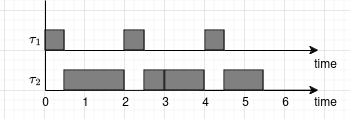
\includegraphics[width=\linewidth, height=100px]{images/schedule_rm.png}
%    a)
%    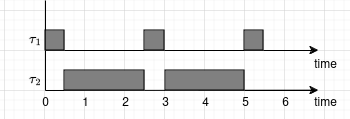
\includegraphics[width=\linewidth, height=100px]{images/schedule_edf.png}
%    b)
%    \caption{Schedules of $\tau_1$ and $\tau_2$ using Rate Monotonic (a)
%    and Earliest Deadline First (b) heuristics.}
%    \label{fig:edf_rm_examples}
%\end{figure}
%
%Although EDF calculates each priority at runtime, it is optimal 
%for uniprocessor scheduling and has a theoretical utilization bound 
%of 1, which is the maximum possible for a feasible taskset on a 
%single processor. RM, on the other hand, has a much lower 
%utilization bound than EDF. While one might argue that RM introduces 
%less runtime overhead and is therefore more practical, it has been 
%shown that RM leads to more task preemptions (interrupting the 
%execution of a task, as seen at times 2 and 4 for task $\tau_2$ in 
%Figure \ref{fig:edf_rm_examples}.a). This, combined with its lower 
%utilization bound and non-optimality, makes EDF perform better than 
%RM\cite{buttazzo2005RMvsEDF}.
%
%Although \cite{liu1973scheduling}'s work focused on uniprocessor 
%systems, the proposed algorithms have also been applied to 
%multi-processor scheduling.
%For example, Global EDF (GEDF)
%can be used on multi-core systems when allowing task migrations
%and Partitioned EDF (PEDF) is used when forbidding task migrations
%(The RM equivalents also exist).